\chapter{Enriched Typing System}

Application of main result (examples and case studies)

\section{Introduction}

\section{Discriminating Two Pure Quantum States}
\todo[inline,size=\normalsize]{pôr introdução a quantum state discrimination e a sua importância e de onde vem a melhor estragegia -> livro Barret}



Given a pure $d$-dimensional state \ket{\psi} known to be either \ket{\psi_0} or \ket{\psi_1}, one must guess which state \ket{\psi} is. In quantum state discrimination, we wish to design a measurement to distinguish optimally between \ket{\psi_0} or \ket{\psi_1}. 

Assume with out loss of generality the angle between \ket{\psi_0}  and \ket{\psi_1}, designated $\alpha$, is between $0$ and $\frac{pi}{2}$. Otherwise, replace \ket{\psi_0} is replaced by $- \ket{\psi_0}$.

In this case the best strategy is is to do the projective measurement with \{\ket{v_0}, \ket{v_1}\}, where \ket{v_0}, \ket{v_1}\ are in the span of \ket{\psi_0}  and \ket{\psi_1} such that $\langle v_{0}| v_{0} \rangle = 0$, they are symmetric with
respect to the angle bisector of \ket{\psi_0}  and \ket{\psi_1}, and \ket{v_i} is closer to  \ket{\psi_i} for $i = 0, 1$. On outcome $“i”$, we guess $\psi_i$.

\begin{figure} [H] 
    \centering
    \begin{center}
        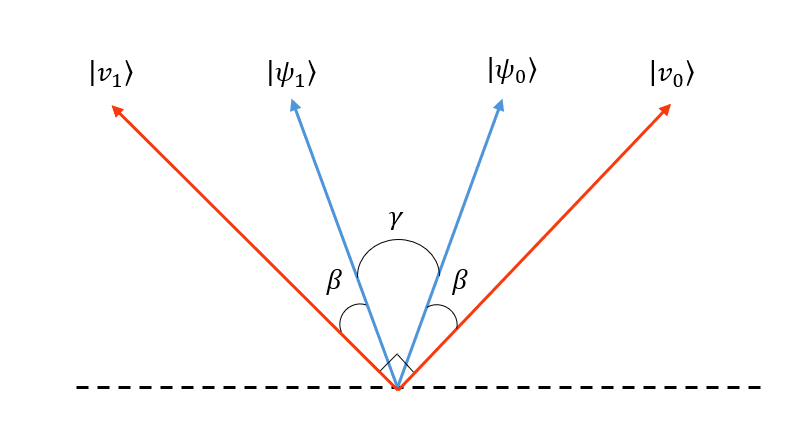
\includegraphics[width=0.6\textwidth]{images/qsd_0.png}
    \end{center}
\caption{Optimal minimum error measurement for discriminating between the pure states \ket{\psi_0}  and  \ket{\psi_1}. This is a
projective measurement onto the states \ket{v_0}  and  \ket{v_1}, symmetrically located on either side of the signal states and shown in red here. $\gamma$ is  the angle between the states \ket{\psi_0}  and  \ket{\psi_1}. $\beta$ is the angle between the states \ket{\psi_0}  and  \ket{v_0} \big/ \ket{\psi_1}  and  \ket{v_1} .}
\label{fig:qsd0}
\end{figure}

The probability of success using the best strategy is

\begin{equation*}
    P_{succ} = \langle \psi_{0}| v_{0} \rangle = \cos^2(\beta) = \cos^2 \left(\frac{\pi/2 - \gamma}{2}\right) = \frac{1}{2} + \frac{1}{2} \cos(\pi/2 -\gamma) = \frac{1}{2} + \frac{1}{2} \sin(\gamma)
\end{equation*}

\subsection{QSD for two pure states: quantum lambda calculus formulation}

Since the quantum lambda calculus presented allows only for explicit projective measurements in the computational basis, it is necessary to rotate the state \ket{\psi} so that \ket{v_0} and \ket{v_1} coincide with the computational basis. This can be done by applying a rotation $R_{\alpha}$ to the state \ket{\psi} such that $R_{\alpha} \ket{v_0} = \ket{0}$. 

\begin{figure} [H] 
    \centering
    \begin{center}
        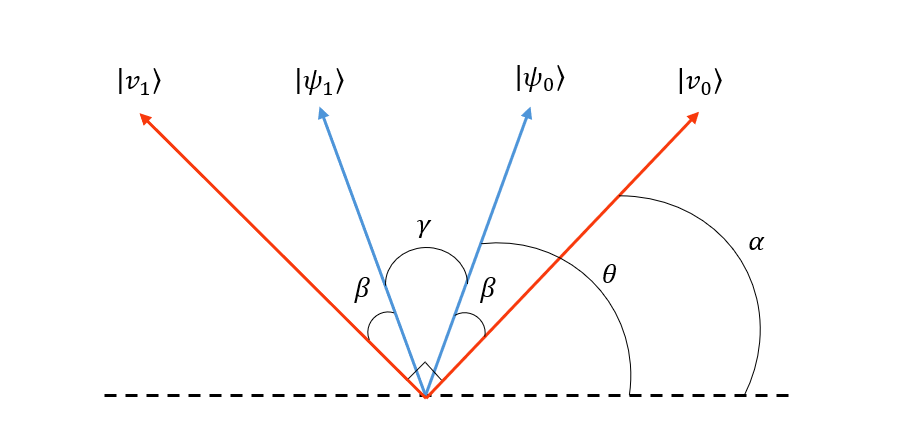
\includegraphics[width=0.6\textwidth]{images/qsd_1.png}
    \end{center}
\caption{Optimal minimum error measurement for discriminating between the pure states \ket{\psi_0}  and  \ket{\psi_1}. $\gamma$ is  the angle between the states \ket{\psi_0}  and  \ket{\psi_1}. $\beta$ is the angle between the states \ket{\psi_0}  and  \ket{v_0} \big/ \ket{\psi_1}  and  \ket{v_1}. $\theta$ is the angle between the states \ket{\psi_0}  and \ket{0} - the polar angle in the Bloch Sphere. $\alpha$ is the angle between the states \ket{v_0}  and \ket{0} .}
\label{fig:qsd1}
\end{figure}

Observing \autoref{fig:qsd1} is possible to conclude that $\alpha = \theta - \beta = \theta - \left(\frac{\frac{\pi}{2}-\gamma}{2} \right) = \theta -  {\frac{\pi}{4}}+\frac{\gamma}{8} $. Given the direction of the rotation, the angle $\alpha$ is negative, so the rotation is $R_{-\alpha}$ which also correspons to $R^{\dag}_{\alpha}$.

As a result, the quantum discrimination for two pure states can be formulated as follows:
\begin{align*}
    q: \textit{qbit}\hspace{3 pt} \triangleright \hspace{3 pt} \textit{meas} (R^{\dag}_{\alpha} (q)) 
 \end{align*}


Attending to \autoref{eq:qubit_bs}, when $q = \ket{\psi_{0}}$ this program is interpreted as follows:

\begin{equation}  \label{eq:teleport_1}
    \begin{split}
  &  \ket{\psi}=   \cos\left(\frac{\theta}{2}\right) \ket{0} + e^{i\phi}\sin\left(\frac{\theta}{2}\right)\ket{1} \\
    \xmapsto{R^{\dag}_{\alpha} (q)} \quad & \left(\cos\left(  \frac{\theta}{2} -  {\frac{\pi}{8}}+\frac{\gamma}{4}\right) \cos\left(\frac{\theta}{2}\right) + \sin\left(\frac{\theta}{2} -  {\frac{\pi}{8}}+\frac{\gamma}{4}\right) e^{i\phi}\sin\left(\frac{\theta}{2}\right) \right)\ket{0}  \\
  & - \left(\sin\left(\frac{\theta}{2} -  {\frac{\pi}{8}}+\frac{\gamma}{4}\right) \cos\left(\frac{\theta}{2}\right)   + \cos\left(  \frac{\theta}{2} -  {\frac{\pi}{8}}+\frac{\gamma}{4}\right) e^{i\phi}\sin\left(\frac{\theta}{2}\right)\right)\ket{1}   \\
  = & \left( \frac{\cos\left(\theta -  {\frac{\pi}{8}}+\frac{\gamma}{4} \right) + \cos\left({-\frac{\pi}{8}}+\frac{\gamma}{4} \right) + e^{i\phi} ( \cos\left({-\frac{\pi}{8}}+\frac{\gamma}{4}\right) - \cos\left(\theta -  {\frac{\pi}{8}}+\frac{\gamma}{4} \right))}{2} \right)   \ket{0}  \\
  & + \left( \frac{-\sin\left(\theta -  {\frac{\pi}{8}}+\frac{\gamma}{4} \right) - \sin\left({-\frac{\pi}{8}}+\frac{\gamma}{4} \right) + e^{i\phi} (\sin\left({\frac{\pi}{8}}+\frac{\gamma}{4}\right) - \sin\left(\theta -  {\frac{\pi}{8}}+\frac{\gamma}{4} \right))}{2}  \right) \ket{1}  \\
  \xmapsto{ \hspace{1pt} \textit{meas} (R^{\dag}_{\alpha} (q))} \quad & \Big( \frac{ \cos^{2}\left(\theta -  {\frac{\pi}{8}}+\frac{\gamma}{4} \right) + \cos\left(\theta -  {\frac{\pi}{8}}+\frac{\gamma}{4}\right)\cos\left( {\frac{\pi}{8}}+\frac{\gamma}{4}\right) + e^{-i\phi} \cos\left(\theta -  {\frac{\pi}{8}}+\frac{\gamma}{4}\right) \cos\left( {\frac{\pi}{8}}+\frac{\gamma}{4}\right) } {4} \\
  & \frac {e^{-i\phi}  \cos^{2}\left(- {\frac{\pi}{8}}+\frac{\gamma}{4} \right) +  } {4}
  &\Big) \\
    \end{split}
  \end{equation}


